\documentclass[conference]{IEEEtran}
\IEEEoverridecommandlockouts
% The preceding line is only needed to identify funding in the first footnote. If that is unneeded, please comment it out.
\usepackage{cite}
\usepackage{amsmath,amssymb,amsfonts}
\usepackage{algorithmic}
\usepackage{graphicx}
\usepackage{textcomp}
\usepackage{xcolor}
\def\BibTeX{{\rm B\kern-.05em{\sc i\kern-.025em b}\kern-.08em
    T\kern-.1667em\lower.7ex\hbox{E}\kern-.125emX}}
\begin{document}

\title{Testing Methodologies for Asynchronous Centralized Simulations\\
}

\author{\IEEEauthorblockN{Sorin Badila, Cale Campbell, Ryan Wilk}
\IEEEauthorblockA{\textit{Department of Computer Science and Engineering} \\
\textit{Oakland University}\\
Rochester, United States \\
sfbadila@oakland.edu, ccampbell5@oakland.edu, rmwilk@oakland.edu}
}

\maketitle

\begin{abstract}
 Distributed interactive multi-body simulations are an increasingly prevalent breed of software and demand unique strategies with respect to testing. 
 Classically non-networked multiplayer video gaming takes place on a single machine hosting a single local environment within which all players directly 
 control actors in a simulation. Modern networked gaming often requires that a singular environment be remotely hosted with all player-controlled actors and 
 their interactions be distributed to connected client applications. With all these simulations, it is paramount that the individual units in the simulations 
 as well as all the moving parts in the server are rigorously tested. The research gathered for this paper will outline the testing methodologies that we find 
 to be the most significant. Combining strong unit and integration testing inside the server, each simulation needs to be tested for usability, compatibility, and 
 reliability. Likewise, since the integrity of the simulation is paramount, susceptibility to malicious or incorrect information fed into the system  must be mitigated, 
 and as such, we will explore mechanisms by which test the system.

\end{abstract}

\begin{IEEEkeywords}
Testing, Nodejs, networking, multiplayer, WebSocket, software engineering
\end{IEEEkeywords}

\section{Introduction}
In our work we aim to create a testing framework for an online multiplayer javascript application called NodeTank. This application involves two primary components, 
a server, and one or more connected clients. Each client instance renders the play environment to the players as well as a tank object and accepts control inputs from 
a player. Client instances are responsible for forwarding control inputs to the server. The server is responsible for tracking and maintaining state information relevant 
to the gameplay. Various examples of state include health status, position, and orientation. This information needs to be forwarded from the server to the client applications 
with minimal latency in order to provide a continuous stream of snapshots of the game’s state. Client applications are also responsible for recreating and displaying this 
information for the player with the end-goal of providing all players with consistent up-to-date information.

Unit testing can be achieved through traditional means of subjecting applicable functions to predetermined inputs and comparing their results to expected results. 
Functional testing presents a less straight-forward solution. In the basic case, there are two clients and one server, three separate processes that are interacting 
with one another. These interactions can potentially generate a very wide range of outputs and behaviors of which only a very small subset would be 
considered correct. Not only do the specific actions and reactions between these processes determine program correctness, but the timing between them determine correctness.

\section{Related Works}

The works of Ariurek et al[2] are very interesting to our research because they propose several mechanisms by which to introduce automated test agents into the game
development cycle with the goal of finding defects. They have proposed two mechanisms by which to facilitate this automation; human-like agents and synthetic agents. 
A human-like agent is a separate program which learns the rules and behavior of a game via reinforcement learning. With reinforcement learning, this type of agent would 
learn how a human would play the game as it would have the same reward incentive as a human player, and is thus likely to detect defects which are similar in nature to those 
detected by humans. Their proposed synthetic agent is also a type of program which is trained via reinforcement learning, except its goals are not inline with the goals of a 
real human player. For example, a synthetic agent could be rewarded with implementing a scenario which would be detrimental to winning the game, but which would be likely to
reveal a defect otherwise hidden from expected behavior. Using both of these methods, Ariurek et al have created a system in which the quality of a game could be tested automatically 
and not in a predetermined fashion. 

Rezin et al[3] developed a model checking mechanism for a specific multiplayer game. They did so by creating a list of attributes which are mapped to parameters into the model -
 for example, each object must have some position identifier, X/Y/Z as well as a vector which describes the orientation. Our case study, NodeTank, will also suffer from the same 
 problem as their case study in that state explosion due the millions of possible position/orientation combinations and as such the game model must be reduced to meaningfully study it. 

Peusaari et al[5] discuss the computational issues and challenges of distributed human-in-the-loop simulations of a basic architecture consisting of several satellite components 
focused around a management component. The specific components include a client, server, motion platform controller, I/O controller, and a manager. The manager distributes setup 
instructions for the simulation as well as collecting and processing data  streams from the other components. The servers play the primary roles of computational units performing 
physics/dynamics processing. The relationship between these client and server components are analogous to the client-server relationship NodeTank utilizes. The piece that we will 
need to construct is the manager, a component that will allow for the distributed initialization of tests and the data collection of those tests. However, in our case, this manager
will observe and report on the behavior code itself rather than sensor data. Components that don’t translate to our work are, with reason, the motion controller. Several of the 
challenges of distributed simulation that are relevant in this paper may be relevant to our work as well. Peusaari outlines the following three main challenges to the distributed 
simulation. The end result of the simulation should be capable of executing in real-time. Secondly, the system, being distributed across a network, will be naturally intolerant of 
delays. The more delay that is introduced, the more the data and validity of the experiment drift. Thirdly data transmissions should be well-planned and organized in such a way that 
minimizes hindrance of the simulation and its core goals. Multi-body simulations require that, at a minimum, coordinates and orientations of bodies subject to physics and dynamics 
calculations be routinely transmitted at reliable intervals.

These are all concerns of our case study, NodeTank. While they may be to a lesser degree, as NodeTank is a game rather than a tool for executing experiments for research, they will be valid concerns
 to the degree of their perceptibility. As delays grow, corresponds to the players’ abilities to enjoy the experience decline.

\section{Background}

Before we may continue to discuss testing methodologies for centralized simulations, we should take a look at what exactly a centralized asynchronous simulation is. 
In this section, we will take a look at the high-level overview of such a simulation before delving into the specific type of data utilized by NodeTank.

\subsection{Architecture}

In attempting to understand the architecture of a centralized simulation, we must also understand under which cirmucstances such an architecture is desired. For example,
let's assume that we have some data that we would like to share between one or more clients, with a client being a receiver which is interested in some data. At a very high level, such
a data sharing layout can be split into two categories: peer-peer and client-server. Smed et. al[6] describes the different layouts in detail, however, generally a peer-peer architecture 
is defined as having two or more clients which have all, or part of some data which is then shared equally each peer. In this scenario, each client is equal to every other client, and thus,
would have to be fully connected to one another[6]. This type of architecture has its own advantages when it comes to certain types of systems, such as file sharing and lock-step simulations,
however we cannot maintain the type of centralized simulation which is pertinent to our topic. 


\subsection{3D Rendering at a High Level}

In the real world, we have object which we can look at and interact with. When such objects are created in a 3D renderer,
some data must be modeled about the object. For simplicity, we will only consider a Cartesian coordinate system(Fig 2), in which points are mapped 
by numerical coordinates along three perpendicular lines(axes). Intuitively, the positional information may be expressed in terms of a displacement 
along each one of the three axes (X, Y, Z). As such, a simple vector with three components can encode this information(Fig 1.): 

\begin{figure}[htbp]
\[ (V_{x}, V_{y}, V_{z}) \]
\caption{Vector Used to Encode Position}
\end{figure}

\begin{figure}[htbp]
\centerline{
\includegraphics [width = 9cm, height = 5cm] {fig1.png}}
\caption{Example of WebGL Coordinate System}
\end{figure}

However, simply listing the poistion is not sufficient in order to accurately map the object in space. An object may be rotated 
around its position. Fig 2. shows a simple example of a car being rotates about the Z axis. The simplest method by which this information can be encoded 
is to use another three component vector to keep track of the roation around each axis, and then apply each rotation to each axis in a cascading fashion. 
This is commonly known as an Euler Angle, which is intuitive to use, but not sufficent enough in our use case due to the possibility of gimbal lock. 
In short terms, gimbal lock can occur when two axes are in a parallel configuration to each other, which would force an otherwise single axis rotation to instead 
become a composite rotation. 


\begin{figure}[htbp]
\centerline{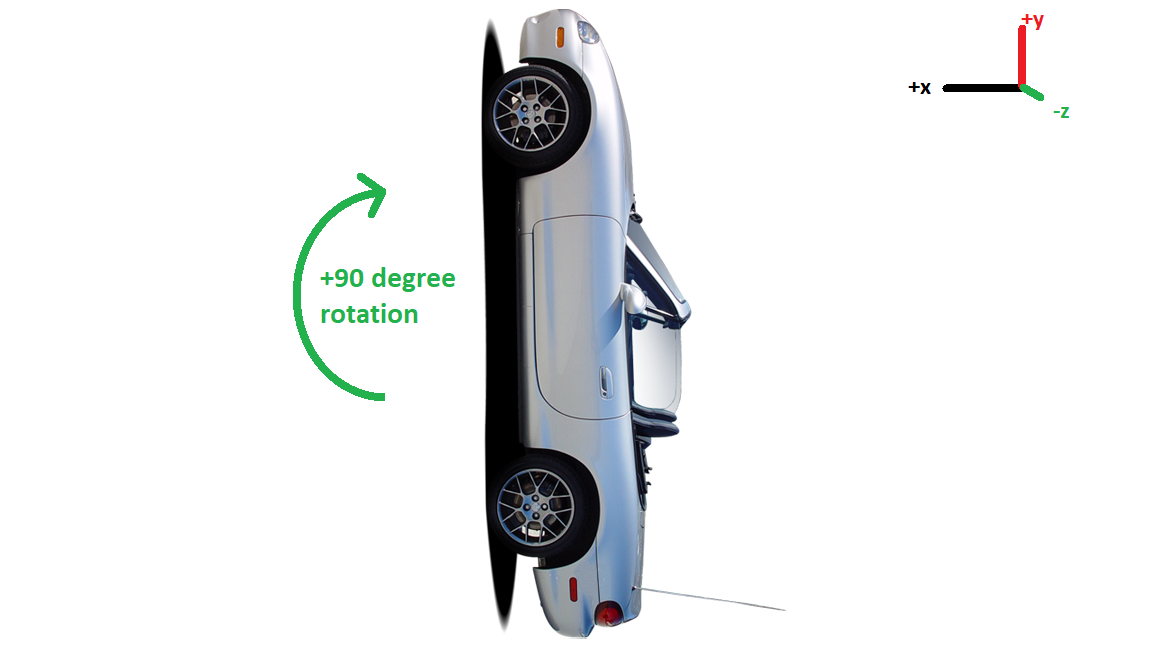
\includegraphics [width = 9cm, height = 5cm] {fig2.png}}
\caption{Example of Rotation Around the Z Axis}
\end{figure}

The conventional solution to this problem is to discard the Euler Angle representation of rotation in favor of using quaternions. 
For the purpose of this paper, we must only know that an equivalent description of orientation can be encoded in a quaternion,
but without the gimbal lock limitation which would cause rotation behavior should it occur. In short, this quaternion may be expressed as a four dimensional
vector, similar to the one expressed in Fig 1., but with an extra component, \textit{w}. 

At this point, we have all of the necessary information to encode a static object in our game world, yet there is one more attribute which
must be implemented: velocity. Consider that an object in our game is in motion, assume it is moving along the X axis. If we have enough snapshots of its location,
then we may be able to render its path up until the current snapshot. However, consider what happens until the next snapshot is received; we will have no idea about the object's path. 
In order to circumvent this, information about how fast the object is moving may be encoded such that an extrapolation between snapshots may occur. This velocity attribute 
is split into two segments; the liear velocity, which is the change in position across the Cartesian system, and angular velocity, which is the change in orientation. 
Each one of these attributes may be encoded in a three dimensional vector(Fig 1).

\begin{figure}[htbp]
\begin{equation}
\text {Position:} (V_{x}, V_{y}, V_{z})
\end{equation}
\begin{equation}
\text {Orientation:} (V_{x}, V_{y}, V_{z}, V_{w})
\end{equation}
\begin{equation}
\text {Linear Velocity:} (V_{x}, V_{y}, V_{z})
\end{equation}
\begin{equation}
\text {Angular Velocity:} (V_{x}, V_{y}, V_{z})
\end{equation}
\caption{Complete Object State}
\end{figure}

Fig 6 shows our final object state. This will be our basic building blokc when we will discuss the protocol in detail, 
as this will become the data packet which updates clients on the state of the simulation and the objects therein. 

\subsection{Game Model}

The protocol workflow has been described at a very high level, but it is agnostic to the specific game and the rules associated with it. The 
player is modeled by a tank object. This tank object has a few properties associated with it: alive, outOfBounds, score. The alive state 
dictates whether the tank is on the playing field - given that in our rules we have established that being shot simply leads to a respawn, 
this state is only used to indicate that a respawn must occur and that the other player's score is incremented. The outOfBounds attribute is true 
when the player steps outside of the game field, which leads to alive being set to false and score being decremented. The score attribute 
keeps track of the player's current score. 

A keen observer would note that a player's tank has many more attributes that those listed above. Rezin et al [3] utilized model checking 
on a multiplayer game, and they came up with an attribute list which contained all variables that would change over the course of the game.
The attributes are tied into parameters, which are constants set at the beginning of the game. For example, a player's tank can be modeled
as a parameter with attrbutes X position, Y position, Z position, lookAt, score, alive, outOfBounds. The limitation of using this approach is that 
if an object's position is utilized in checking the model, the list of all possible state combinations would be too large to ever compute due 
to the size of the game field having granularity in the tens of millions and the total number of possible lookAt locations also being in the millions.

With these considerations in mind, model checking has also been overlooked in favor of utilizing automated testing to test the 
game directly for consistency in its rules. One thing of note is that the formal definition of the game rules for example, a valid x coordinate,
is syntactically equivalent to the check the game logic would perform; therefore writting a model checking program is redundant in this specific 
case. Fig 11 shows the formal definition along with the implementation of the rule. 

\begin{figure}[htbp]
\[ (W_{xmin} \leq T_{x} \leq W_{xmax}) \]
\[ !(playerTanks[k].obj.position.x < xMin ||\]
\[ playerTanks[k].obj.position.x > xMax) \]
\caption{Formal Rule and Implementation of Valid X coordinate}
\end{figure}

\section{Approach}
Our approach is to develop a testing framework for NodeTank will combine abstract testing of models, unit testing, and functional testing into a single, yet modular, 
utility. The effort of functional testing will involve the synchronization of timing of outputs from the server as well as the clients involved. The testing utility 
should be distributable just as the software being tested and a means of distributing and launching a test should be runnable from a single test location. Any data and 
any results of a test run should also be collected and delivered to the single test location where it will be analyzed and classified as either a success or failure. 
Current design will feature the integration of the Labstreaminglayer tool and a Labstreaminglayer server. This tool will allow for the collection of any data or output 
deemed necessary for a given test. It will allow for record sub-millisecond timing of events from multiple machines over a local area network.

For the goal of developing and testing the game locally on one machine, we will also be able to leverage the fact that it is built to run in the browser on
an interpreted language to run test suites end to end. Firstly, we will investigate an approach similar to Ariyurek et al[2] in order to develop an automated 
system to test the application as well as to automatically find problems with it. Secondly, the fact that the application in its unobstructed build state will have
its internal state visible and inspectable from the outside. That is to say, if we were to run multiple client simulations concurrently, we would be able to inspect 
the state of the simulation on each one of the said client machines independently. This would allow us to inspect the correctness of the model in real time from the 
perspective of each client. Likewise, the fact that we could control each client independently, we will be able to gauge the susceptibility of the simulation to erroneous 
or malicious data by willfully introducing it to one client, and checking if the erroneous data was propagated to the other clients.


\section{Implementation}

With the all of the prerequisite work complete, the implementation of the the game and protocol will be discussed. For reference,
the project code is located at (https://github.com/spac3nerd/CSI-5390Proj). The nodejs server 
will need to run both traditional HTTP transactons and socket transactions. The HTTP transactions are used to ask the server if 
there are any open spots in the game, and whether access is granted to a new player. If access is granted, then the server will return 
an unique token to the client with which a socket connection can be requested. The client then requests entry into the game 
with the token and a tunnel is established between the client and the server. 

In the following sections we will cover the specific testing implementations with the goal of addressing the problem of rigorously testing NodeTank, or any 
other multiplayer game built on the NodeJS platform. 


\subsection{Automated Functional Testing}

The first testing scenario we will consider is to allow the system to automatically play the game in order to test a set of pre-defined set of actions.
For example, we can programatically interact with the game directly in order to control one of the player tanks. With the system having control over a player character, 
we can individually test the different aspects of the game: movement, shooting, respawning etc... This type of autmated testing could be invoked on an individual developer's 
machine in order to test each function of the game as its being developed. 

However, we may take this testing even further and consider that since the game runs within the browser, we would be able to tap into any concurrent client simulation. This 
has the implication that we would be able to inspect the state of each client concurrently. 

\subsection{Automated Unit Testing}

To be developed 


\subsection{Trained Model Approach}

Discuss the setup for the trained model - the tools and automatic invocation


\section{Case Study}

Discuss the specificics of the game architecture here - show the actual code and frameworks


\section{Conclusion}

To be developed 

\section{References}
[1] A. Valadares, “Aspect-oriented architectural style for distributed interactive simulations”, 2016, 
Available from ProQuest Dissertations & Theses Global. (1881527059). 
Retrieved from https://search-proquest-com.huaryu.kl.oakland.edu/docview/1881527059?accountid=12924

[2] S. Ariyurek, “Automated Video Game Testing Using
Synthetic and Human-Like Agents”, 2019, Available: https://arxiv.org/pdf/1906.00317.pdf
	
[3] R. Rezin, ”Model Checking in multiplayer games development”, Innopolis University, 
2017, Available: https://arxiv.org/pdf/1712.01207.pdf

[4] R. Hofer “DIS Today”, 1995, Available:
https://ieeexplore.ieee.org/stamp/stamp.jsp?arnumber=400453

[5] J.Peusaari, “Distributed Issues in Real-Time Interactive Simulations”, Department of Technology Lappeenranta University of Technology, Finland,
 Available: https://ieeexplore.ieee.org/abstract/document/5361761
 
[6] J. Smed, "Aspects of Networking in Multiplayer Computer Games", Proceedings of International Conference on Application and Development of Computer Games in the 21st Century, Hong Kong, 2001,
Available: https://www.researchgate.net/publication/269251176_Aspects_of_Networking_in_Multiplayer_Computer_Games
\end{document}
